
\documentclass[pdflatex,sn-mathphys-num]{sn-jnl}% 

\usepackage{graphicx}%
\usepackage{multirow}%
\usepackage{amsmath,amssymb,amsfonts}%
\usepackage{amsthm}%
\usepackage{mathrsfs}%
\usepackage[title]{appendix}%
\usepackage{xcolor}%
\usepackage{textcomp}%
\usepackage{manyfoot}%
\usepackage{booktabs}%
\usepackage{algorithm}%
\usepackage{algorithmicx}%
\usepackage{algpseudocode}%
\usepackage{listings}%
\usepackage{tabularx}
\usepackage{ragged2e}
\usepackage{placeins}
\usepackage{float}
\usepackage[justification=centering]{caption}

%%%%

%%%%%=============================================================================%%%%

%%%%%=============================================================================%%%%

%% as per the requirement new theorem styles can be included as shown below
\theoremstyle{thmstyleone}%
\newtheorem{theorem}{Theorem}%  meant for continuous numbers
%%\newtheorem{theorem}{Theorem}[section]% meant for sectionwise numbers
%% optional argument [theorem] produces theorem numbering sequence instead of independent numbers for Proposition
\newtheorem{proposition}[theorem]{Proposition}% 
%%\newtheorem{proposition}{Proposition}% to get separate numbers for theorem and proposition etc.

\theoremstyle{thmstyletwo}%
\newtheorem{example}{Example}%
\newtheorem{remark}{Remark}%

\theoremstyle{thmstylethree}%
\newtheorem{definition}{Definition}%

\raggedbottom
%%\unnumbered% uncomment this for unnumbered level heads

\begin{document}

\title{Machine Learning Meets Digital Empathy: A Holistic Approach to Cyberbullying Detection}

%%=============================================================%%
%% GivenName	-> \fnm{Joergen W.}
%% Particle	-> \spfx{van der} -> surname prefix
%% FamilyName	-> \sur{Ploeg}
%% Suffix	-> \sfx{IV}
%% \author*[1,2]{\fnm{Joergen W.} \spfx{van der} \sur{Ploeg} 
%%  \sfx{IV}}\email{iauthor@gmail.com}
%%=============================================================%%

\author{\fnm{Aranya} \sur{Jana}\textsuperscript{1[\texttt{\orcidID{0009-0007-0189-6012}}]}}%%\email{iauthor@gmail.com}

\author{\fnm{Arindam} \sur{Sahoo}\textsuperscript{1[\texttt{\orcidID{0009-0001-9952-1935}}]}}%%\email{iiiauthor@gmail.com}

\author{\fnm{Abir} \sur{Nath}\textsuperscript{1[\texttt{\orcidID{0009-0008-2597-0747}}]}}%%\email{iiauthor@gmail.com}

\author{\fnm{Sujata} \sur{Mondal}\textsuperscript{1[\texttt{\orcidID{0009-0000-8244-5166}}]}}%%\email{iiiauthor@gmail.com}

\author{\fnm{Tanmoy} \sur{Ghosh}\textsuperscript{1[\texttt{\orcidID{0000-0002-5479-5465}}]}}%%\email{iiiauthor@gmail.com}

\author{\fnm{Dishani} \sur{Roy}\textsuperscript{1[\texttt{\orcidID{0009-0008-8879-6109}}]}}%%\email{iiiauthor@gmail.com}

\affil[1]{\orgname{Narula Institute of Technology}, \city{Kolkata}, \state{West Bengal}, \country{India}}


%%==================================%%
%% Sample for unstructured abstract %%
%%==================================%%

% \abstract{A cyberbully is an emerging risk of digital communities whose existence requires creating a trustworthy system for the detection and protection of mental health. Solving this issue is achieved using a combination of sophisticated machine learning methods and understanding from neurobiology. Convolutional Neural Networks (CNNs) and Augmented BERT are used in processing large volumes of social network data, outperforming all existing approaches through improved precision and recall. The model facilitates real-time monitoring, which allows for quicker responses to harassment incidents. Using large amounts of data from online interactions helps achieve a better picture of cyberbullying trends and behavioral patterns. Another part of this problem concerns the adverse effect of cyberbullying on human brain neurobiology, with suggested prevention and intervention strategies. Knowledge of the psychological processes behind such behavior informs more effective education and support interventions for those who are affected.Fostering a culture of respect and empathy in online environments is also identified as one of the determinants of decreased levels of cyberbullying prevalence. These results suggest the need for technological innovation and inter-disciplinary strategy in addressing the effects of cyberbullying.}

\abstract{A cyberbully is an emerging risk of digital communities whose existence requires creating a trustworthy system for the detection and protection of mental health. The resolution of this problem necessitates both technological advancements in addition to psychological comprehension. Our research develops a combined cyberbullying detection system which uses Convolutional Neural Networks (CNNs) along with a transformer-based BERT network that processes extensive multilingual social media content. The model supports English and Hindi and Bengali as well as their combinations (Hinglish and Benglish) for processing content to detect cyberbullying with cultural awareness and language adaptiveness. This harassment system maintains instantaneous analysis methods and contains emotion and sentiment detection elements that boost model comprehension of user intentions and situational context. Researchers found cyberbullying creates psychological harm in their investigations and indicated that uniting behavioral comprehension with technological solutions could develop secure online environments with higher empathy. The study proven that successful cyberbullying prevention requires integrating machine learning with mental health methods as new tools to fight against modern cyberbullying cases.}

%%================================%%
%% Sample for structured abstract %%
%%================================%%


\keywords{Cyberbullying, Detection System, Machine Learning, BERT, Text Analysis, Social Media, NLP}

%%\pacs[JEL Classification]{D8, H51}

%%\pacs[MSC Classification]{35A01, 65L10, 65L12, 65L20, 65L70}

\maketitle
\clearpage
\section{Introduction}\label{sec1}

Extensive social communication opportunities are currently delivered through digital platforms via social media as one of the dominant trends of the time. The digital devices uniting Facebook, Instagram, TikTok and Twitter users across four billion five hundred million worldwide individuals produce cyberbullying as a destructive result of electronic social interactions that affects young people especially.\cite{bib7}\cite{bib8} Victims of cyberbullying encounter concentrated digital attacks through practices like social isolation followed by intentional harassment and identity deception.  Virtual means provide sustenance to those who commit harmful actions because of the combination between geographical distance and anonymous interactions which enables their harmful behavior to persist without direct consequences.

Research indicates that between 15 and 20 percent of kids experience some form of online harassment, which is a startlingly high prevalence of cyberbullying. \cite{bib7}  The victim may experience severe emotional and psychological effects, often including elevated anxiety, sadness, and, in severe situations, suicide thoughts. \cite{bib21}  Beyond issues of personal health, the pervasiveness of cyberbullying ruins peer relationships\cite{bib1}, alters social dynamics, and fosters a toxic environment that can impede academic achievement and personal development.  The necessity of effective detection and intervention systems becomes crucial because of their vital role.

Manual reporting and keyword scanning systems used to detect cyberbullying prove inadequate because they cannot identify advanced forms of cyber harassment documented in references 9 and 10. Traditional detection systems fail at interpreting social media communication since they lack the capability to decode the hidden abusive messages that use coded expressions combined with slang and emoji language\cite{bib8}. The detection of cyberbullying becomes difficult because victims do not report incidents and detection systems cannot view the lowest possible intensity of cyberbullying scenarios. The victims remain unprotected when no support measures are in place. Current detection systems fail to prevent cyberbullying completely which proves the urgent necessity for improved systems that can recognize abuse events. 

The research develops a detection system with advanced ML and DL methods to address this pivotal problem. A fast-acting, aggressive social media analytics system has been developed through the combination of text and image processing approaches. This system provides real-time reporting along with alert capabilities to enable both victims and moderators to swiftly act upon cyberbullying incidents, thereby safeguarding people from such damage.

This investigation produces results that surpass detection methods by advancing the security of online environments for multiple user groups. Detection strategies aim to develop equal offerings in digital space while recognizing both data-management moral concerns and changing online interaction dynamics. Collaboration among scientific researchers, practitioners, and social media companies is necessary to stop cyberbullying, as this activity represents an essential social responsibility. Joint efforts in fighting online harassment produce optimal results when communities unite to develop supportive spaces in digital environments.



\section{Literature Study}\label{sec2}
The detection of cyberbullying on social media, including school groups\cite{bib7}\cite{bib1} and professional networks has become a prominent research topic because of increasing online harassment effects on mental health. Multiple researchers investigate various approaches starting with rule-based methodologies through advanced ML and DL techniques, according to reference \cite{bib2}. The second segment analyzes critical studies together with their research approaches and challenges, and unaddressed areas.


\subsection{Survey on various Detection Techniques}

% \bigskip
{
\scriptsize
\begin{tabular}{|p{1.5cm}|p{2.5cm}|p{2.5cm}|p{2.5cm}|p{2.5cm}|p{2.5cm}|}
\hline
\textbf{Authors} & \textbf{Methodology} & \textbf{Result/ Findings} & \textbf{Source/ Dataset} & \textbf{Research Gap} \\
\hline
% Nakov, Preslav, et al. \cite{bib8} & The paper surveys datasets for abusive language detection, citing Kaggle, Hatebase, Founta, and Davidson. & The paper surveys datasets for abusive language detection, citing Kaggle, Hatebase, Founta, and Davidson. & The paper surveys datasets for abusive language detection, citing Kaggle, Hatebase, Founta, and Davidson. & The paper surveys datasets for abusive language detection, citing Kaggle, Hatebase, Founta, and Davidson. \\
% \hline
Isabella Kamanthi, P. \cite{bib7} & Highlights serious mental health impact, with students reporting high victimization and perpetration rates, leading to anxiety and depression. & Highlights serious mental health impact, with students reporting high victimization and perpetration rates, leading to anxiety and depression. & Highlights serious mental health impact, with students reporting high victimization and perpetration rates, leading to anxiety and depression. & Highlights serious mental health impact, with students reporting high victimization and perpetration rates, leading to anxiety and depression. \\
\hline
Orr, Taaj Weraphorn \cite{bib1} & Further research needed on negative emotions' impact on cyberbullying and protective factors like peer relationships. & Further research needed on negative emotions' impact on cyberbullying and protective factors like peer relationships. & Further research needed on negative emotions' impact on cyberbullying and protective factors like peer relationships. & Further research needed on negative emotions' impact on cyberbullying and protective factors like peer relationships. \\
\hline
Dadvar, Maral, et al. \cite{bib2} & This dataset comprises 4,626 comments from YouTube manually labelled for bullying and was posted by 3,858 different users. & This dataset comprises 4,626 comments from YouTube manually labelled for bullying and was posted by 3,858 different users. & This dataset comprises 4,626 comments from YouTube manually labelled for bullying and was posted by 3,858 different users. & This dataset comprises 4,626 comments from YouTube manually labelled for bullying and was posted by 3,858 different users. \\
\hline
Zhang, Xiang, and Yann LeCun \cite{bib3} & Employs several large-scale datasets, such as Yahoo! Answers, Amazon reviews, and DBpedia ontology classification, to ensure diverse text samples.
 & Employs several large-scale datasets, such as Yahoo! Answers, Amazon reviews, and DBpedia ontology classification, to ensure diverse text samples.
 & Employs several large-scale datasets, such as Yahoo! Answers, Amazon reviews, and DBpedia ontology classification, to ensure diverse text samples.
 & Employs several large-scale datasets, such as Yahoo! Answers, Amazon reviews, and DBpedia ontology classification, to ensure diverse text samples.
 \\
\hline
\end{tabular}

\begin{tabular}{|p{1.5cm}|p{2.5cm}|p{2.5cm}|p{2.5cm}|p{2.5cm}|p{2.5cm}|}
\hline
\textbf{Authors} & \textbf{Methodology} & \textbf{Result/ Findings} & \textbf{Source/ Dataset} & \textbf{Research Gap} \\
\hline
MacAvaney, Sean, et al. \cite{bib5} & This work proposes a multi-view SVM approach, with the emphasis on simplicity and interpretability, and applies TF-IDF features from text data. & This work proposes a multi-view SVM approach, with the emphasis on simplicity and interpretability, and applies TF-IDF features from text data. & This work proposes a multi-view SVM approach, with the emphasis on simplicity and interpretability, and applies TF-IDF features from text data. & This work proposes a multi-view SVM approach, with the emphasis on simplicity and interpretability, and applies TF-IDF features from text data. \\
\hline
Kovács, György, Pedro Alonso, and Rajkumar Saini \cite{bib6} & The primary dataset used is the HASOC 2019 training set, supplemented by various external labeled corpora and pretrained word embeddings. & The primary dataset used is the HASOC 2019 training set, supplemented by various external labeled corpora and pretrained word embeddings. & The primary dataset used is the HASOC 2019 training set, supplemented by various external labeled corpora and pretrained word embeddings. & The primary dataset used is the HASOC 2019 training set, supplemented by various external labeled corpora and pretrained word embeddings. \\
\hline
Sathya Devi M., Dr.Indira B., Vinayak M.S., Vinay B.S. \cite{bib4} & Demand: efficient detection in diverse languages and integration of psychological insights into detection algorithms. & Demand: efficient detection in diverse languages and integration of psychological insights into detection algorithms. & Demand: efficient detection in diverse languages and integration of psychological insights into detection algorithms. & Demand: efficient detection in diverse languages and integration of psychological insights into detection algorithms. \\
\hline
Fati, Suliman Mohamed, et al. \cite{bib9} & Highlights the need for standardized datasets and multilingual approaches in cyberbully detection research. & Highlights the need for standardized datasets and multilingual approaches in cyberbully detection research. & Highlights the need for standardized datasets and multilingual approaches in cyberbully detection research. & Highlights the need for standardized datasets and multilingual approaches in cyberbully detection research. \\
\hline
Islam, Md Manowarul, et al. \cite{bib10} & Texts about bullying posted on social media websites such as Facebook and Twitter to train and test the approach.
 & Texts about bullying posted on social media websites such as Facebook and Twitter to train and test the approach.
 & Texts about bullying posted on social media websites such as Facebook and Twitter to train and test the approach.
 & Texts about bullying posted on social media websites such as Facebook and Twitter to train and test the approach.
 \\
\hline
\end{tabular}

\begin{tabular}{|p{1.5cm}|p{2.5cm}|p{2.5cm}|p{2.5cm}|p{2.5cm}|p{2.5cm}|}
\hline
\textbf{Authors} & \textbf{Methodology} & \textbf{Result/ Findings} & \textbf{Source/ Dataset} & \textbf{Research Gap} \\
\hline
Vora, Deepali, et al. \cite{bib11} & Study addresses gaps by introducing attention mechanisms and advanced feature extraction for improved accuracy. & Study addresses gaps by introducing attention mechanisms and advanced feature extraction for improved accuracy. & Study addresses gaps by introducing attention mechanisms and advanced feature extraction for improved accuracy. & Study addresses gaps by introducing attention mechanisms and advanced feature extraction for improved accuracy. \\
\hline
Kumar, Akshi, and Nitin Sachdeva \cite{bib12} & Bi-LTSM + Attention + CapsNet gave accuracy 92.67\% and above, Bi-GRU + Attention + CapsNet gave accuracy of 93.89\% and above and Bi-GRU + Attention + CNN gave accuracy of 91.83\% and above. & Bi-LTSM + Attention + CapsNet gave accuracy 92.67\% and above, Bi-GRU + Attention + CapsNet gave accuracy of 93.89\% and above and Bi-GRU + Attention + CNN gave accuracy of 91.83\% and above. & Bi-LTSM + Attention + CapsNet gave accuracy 92.67\% and above, Bi-GRU + Attention + CapsNet gave accuracy of 93.89\% and above and Bi-GRU + Attention + CNN gave accuracy of 91.83\% and above. & Bi-LTSM + Attention + CapsNet gave accuracy 92.67\% and above, Bi-GRU + Attention + CapsNet gave accuracy of 93.89\% and above and Bi-GRU + Attention + CNN gave accuracy of 91.83\% and above. \\
\hline
Al-Ajlan, Monirah Abdullah, and Mourad Ykhlef \cite{bib13} & Dataset comprised of 39,000 tweets retrieved from Twitter streaming API, labeled by human intelligence concerning bullying content.
 & Dataset comprised of 39,000 tweets retrieved from Twitter streaming API, labeled by human intelligence concerning bullying content.
 & Dataset comprised of 39,000 tweets retrieved from Twitter streaming API, labeled by human intelligence concerning bullying content.
 & Dataset comprised of 39,000 tweets retrieved from Twitter streaming API, labeled by human intelligence concerning bullying content.
 \\
\hline
Akhter, Muhammad Pervez, et al. \cite{bib14} & Uses conventional machine learning and deep learning models like CNN, LSTM, BLSTM, and CLSTM for comment classification into abusive and non-abusive.

 & Uses conventional machine learning and deep learning models like CNN, LSTM, BLSTM, and CLSTM for comment classification into abusive and non-abusive.

 & Uses conventional machine learning and deep learning models like CNN, LSTM, BLSTM, and CLSTM for comment classification into abusive and non-abusive.

 & Uses conventional machine learning and deep learning models like CNN, LSTM, BLSTM, and CLSTM for comment classification into abusive and non-abusive.

 \\
\hline
Qiu, Jiabao, Melody Moh, and Teng-Sheng Moh \cite{bib15} & Twitter API.
 & Twitter API.
 & Twitter API.
 & Twitter API.
 \\
\hline
\end{tabular}

\begin{tabular}{|p{1.5cm}|p{2.5cm}|p{2.5cm}|p{2.5cm}|p{2.5cm}|p{2.5cm}|}
\hline
\textbf{Authors} & \textbf{Methodology} & \textbf{Result/ Findings} & \textbf{Source/ Dataset} & \textbf{Research Gap} \\
\hline
Mioara, Boca-Zamfir \cite{bib16} & Lack of focus on social networking site cyberbullying, aspect-based analysis, and advanced classifier integration. & Lack of focus on social networking site cyberbullying, aspect-based analysis, and advanced classifier integration. & Lack of focus on social networking site cyberbullying, aspect-based analysis, and advanced classifier integration. & Lack of focus on social networking site cyberbullying, aspect-based analysis, and advanced classifier integration. \\
\hline
Paul, Sayanta, Sriparna Saha, and Mohammed Hasanuzzaman \cite{bib17} & Trained on limited training data. & Trained on limited training data. & Trained on limited training data. & Trained on limited training data. \\
\hline
Shakeel, Nida, and Rajendra Kumar Dwivedi\cite{bib18} & Highest accuracy of 92.6\% is achieved using Logistic Regression. & Highest accuracy of 92.6\% is achieved using Logistic Regression. & Highest accuracy of 92.6\% is achieved using Logistic Regression. & Highest accuracy of 92.6\% is achieved using Logistic Regression. \\
\hline
Toktarova, Aigerim, et al.\cite{bib19} & The arms race highlights the need for improved detection technologies and more research in cyberbully detection. & The arms race highlights the need for improved detection technologies and more research in cyberbully detection. & The arms race highlights the need for improved detection technologies and more research in cyberbully detection. & The arms race highlights the need for improved detection technologies and more research in cyberbully detection. \\
\hline
Esha et.al.\cite{bib20} & Low recall in insult detection, ineffective classification, and need for improved NLP learning strategies for cyberbullying. & Low recall in insult detection, ineffective classification, and need for improved NLP learning strategies for cyberbullying. & Low recall in insult detection, ineffective classification, and need for improved NLP learning strategies for cyberbullying. & Low recall in insult detection, ineffective classification, and need for improved NLP learning strategies for cyberbullying. \\
\hline
Rabani S.T., Khan Q.R. and Akib K.\cite{bib21} & Data collected from Twitter, tweets pre-processed and manually annotated, with ML and ensemble methods for classification. & Data collected from Twitter, tweets pre-processed and manually annotated, with ML and ensemble methods for classification. & Data collected from Twitter, tweets pre-processed and manually annotated, with ML and ensemble methods for classification. & Data collected from Twitter, tweets pre-processed and manually annotated, with ML and ensemble methods for classification. \\
\hline
\end{tabular}
}
\bigskip

\\Isabella Kamanthi, P. \cite{bib7}
The combination of being a victim and abuser exposes students to higher risks of developing depression and anxiety so researchers emphasize the requirement for improved whole-school bullying prevention strategies.

\\Orr, Taaj & Weraphorn. \cite{bib1}
Researchers analyzed cyberbullying across demographics using surveys; findings suggest future studies explore emotional impact and peer protection roles in such cases.

\\Dadvar, Maral, et al. \cite{bib2}
Supervised classification received training through all three features including content and specific cyberbullying indicators along with user attributes. A user context addition to the system detected cyberbullying in 4,626 manual reviews of YouTube comments from 3,858 users while reaching 77\% precision and 55\% recall.

% \\Zhang, Xiang, and Yann LeCun \cite{bib3} 
% Temporal convolutional networks serve as the analytical tools during ontology classification and sentiment analysis while eliminating standard linguistic approaches. Using large-scale datasets like Yahoo! The methods applied their algorithms on Yahoo! Answers combined with Amazon reviews and DBpedia and produced accuracy between 59.16\% and 98.27\%. The research underlines how big and professional datasets and easily accessible resources play a vital role in performing text understanding effectively.

\\MacAvaney, Sean, et al. \cite{bib5}
Research investigators relied on SVM to process multi-view TF-IDF features which yielded 80\% Stormfront success and 53.68\% TRAC macro F1 while exceeding all existing techniques. The research focused on both data selection procedures and enhanced understanding methods.

\\Kovacs, Gyorgy, Pedro Alonso, and Rajkumar Saini \cite{bib6}
Through BERT variants alongside external linguistic databases the scientists achieved 0.7953 macro F1 and 0.8498 weighted F1 results on HASOC 2019. The research conducted shows that additional hate speech definitions together with larger labeled datasets would advance understanding.

% \\Sathya Devi M., Dr. Indira B., Vinayak M.S., Vinay B.S. \cite{bib4}
% The model utilized ensemble learning combined with deep CNNs to analyze text and video contents for detecting harassment. The detection system reached F1-scores between 0.85 and 0.97 throughout the analysis of four cyberbullying classifications. The author used Twitter together with video data while recommending psychological elements for inclusion in detection systems.

\\Fati, Suliman Mohamed, et al. \cite{bib9}
A Conv1DLSTM model with attention achieved 86.49\% accuracy, 81.46\% precision, 89.19\% recall, and 85.15\% F1-score on 37,373 tweets. The study urges standardized, multilingual datasets.

Islam, Md Manowarul, et al. \cite{bib10}
Research demonstrated NLP and ML models where SVM reached more than 75\% success rate for recognizing cyberbullying. Current Facebook and Twitter multilingual detection systems need improvement according to the obtained monitoring results.

\\Vora, Deepali, et al. \cite{bib11}
The authors used deep learning with attention mechanisms alongside word2vec CBOW features and Conv1DLSTM classifier to reach 94.03\% accuracy when analyzing Twitter data globally.

% \\Kumar, Akshi, and Nitin Sachdeva \cite{bib12}
% The applied sequence of Bi-GRU + Attention + CapsNet produced 93.89\% accuracy in the model performance. The study analyzed difficulties when working with multilingual and multimodal datasets through using data from Formspring.me and MySpace.

% \\Al-Ajlan, Monirah Abdullah, and Mourad Ykhlef \cite{bib13}
% A CNN-CB model in the study reached 95\% accuracy and 93\% precision while processing the 39,000 documented tweets. The research focuses on emphasizing the necessity of developing sophisticated algorithms to address the new methods used in cyberbullying.

\\Akhter, Muhammad Pervez, et al. \cite{bib14}
Research evaluated deep learning models (CNN, LSTM, BLSTM, CLSTM) and traditional ML approaches for abusive language detection while deep learning surpassed 90\% accuracy through use of Urdu and Roman Urdu datasets to handle sparse datasets.

\\Qiu, Jiabao, Melody Moh, and Teng-Sheng Moh \cite{bib15}
Using CNN and Tensor Fusion Network together with VGG-19 helped the study achieve 89\%–92\% accuracy when processing text and metadata from Twitter API though some irrelevant attributes were present.

\\Mioara, Boca-Zamfir \cite{bib16}
Habit key scored 0.67 under pre-processing that applied TF-IDF and SVM classifiers according to this study despite its lack of focus on social media and advanced analysis models.

\\Paul, Sayanta, Sriparna Saha, and Mohammed Hasanuzzaman \cite{bib17}
Applied Universal Sentence Encoder, Transformer Encoder, ResBiLSTM, and Recurrent CNN. The system demonstrated a success rate between 47-69\% when identifying bullies along with 72-87\% achievement in detecting non-bullies. Data collected from Vine. Limited by small training datasets.

% \\Shakeel, Nida, and Rajendra Kumar Dwivedi \cite{bib18}
% The research used SVM and Logistic Regression models which led to 92.6\% accuracy from the Logistic Regression model. The analyzed comments originated from Twitter as well as Facebook and YouTube. Machine learning methods used for this study were restricted to supervised execution series.

\\Toktarova, Aigerim, et al. \cite{bib19}
The research demonstrated how deep learning models including LSTM, BiLSTM and CNN outperformed shallow models with Word2Vec and GloVe and provided higher F1-scores reaching up to 0.899. Cyberbullying detection methods need enhancement according to this research and scientists require additional investigation.

\\Esha et al. \cite{bib20}
The research team used NLP along with ML-based aggressive language detection methods. The accuracy rates obtained by using Logistic Regression and Random Forest exceeded other methods but remained between 0.50 and 0.53 due to difficulties detecting insults. Dataset details were missing.

% \\Rabani S.T., Khan Q.R. and Akib K. \cite{bib21}
% Researchers retrieved tweets from Twitter as part of their work which they cleaned then manually assigned classes. Random Forest ensemble demonstrated 98.5\% accuracy as well as 98.7\% precision when identifying suicidal from non-suicidal tweets. Lacked predictive and intervention capabilities.
\\Text-based detection of cyberbullying is the most common approach used in the literature. Several machine learning and deep learning techniques have been employed for classifying abusive and non-abusive content in text form. 
    \item
    \textbf{Machine Learning Approaches:}
    Machine learning (ML) techniques, including Naive Bayes, Support Vector Machines (SVM), and Decision Trees, have been widely used for cyberbullying detection.\cite{bib3} These models rely on handcrafted features such as word frequencies, syntactic structures, and sentiment scores to detect bullying behavior. A notable example is the work of Dadvar et al. (2013)\cite{bib2}, who applied a SVM classifier to identify cyberbullying comments on Twitter, achieving a classification accuracy of 80\%. While effective, these models often struggle with scalability and generalizability to large datasets, especially when the data is noisy or unstructured.
\subsection{Data Analysis}
\subsubsection{Data Preprocessing}
% The research dataset contained two main columns with text comments and their relevant classification labels. The label system specified both the presence of cyberbullying and which category of abuse applied from among age, race, gender or religion. The analysis included remarks designated as not\_cyberbullying as well as abusive content.

% The labeling scheme received a one-hot encoded transformation into a six-column format of text as well as age, race, gender, not\_cyberbullying, and religion for multi-label classification and better interpretability through analysis and model training.

% The relevant category received a value of 1 while every other category in each entry received a value of 0. If a comment belonged to the category of gender analysts set the gender column at value 1 and every other class column at value 0. The comments flagged as not\_cyberbullying received a single 1 in the specific column of marking as the remaining classification categories became 0.

% The modification allowed the dataset to handle two classification tasks simultaneously with binary and multi-class structure through simplified assessment processes.

% The dataset consisted of user comments labeled either as \texttt{not\_cyberbullying} or with one of several cyberbullying categories: \texttt{age}, \texttt{race}, \texttt{gender}, \texttt{religion}.  The six binary columns were derived from the original label column in order to represent each possible category. The single-point value of one was assigned to the relevant category field and all other fields received a value of zero for each row.

The dataset included text comments categorized into cyberbullying types that were grouped into age groups, racial identities, gender identities, religious backgrounds together with non-cyberbullying text labels. The data received one-hot encoding across five categories which included text, age, race, gender and religion and not cyberbullying by setting 1 for relevant categories while the others were set to 0. The defined structure permitted one framework to conduct both binary and multi-class classification operations.

The \texttt{text} column underwent preprocessing which combined successive spaces into one space while stripping mentions and URLs, HTML tags and Unicode characters and transformed text into lowercase. The implemented standardization methods decreased both numerical and processing errors and bias during the processing step.

This research required multilingual compatibility so synthetic data augmentation using back-translation and transliteration produced replicas of Hinglish, Benglish, Hindi, and Bengali content types. The processing system used FastText for language identification purposes to route data according to specific linguistic needs. The preprocessing step relied on multilingual BERT-compatible tokenizers for tokenization before performing language-specific stopword removal during both English and Indic language processing.

\begin{figure}[H]
    \centering
    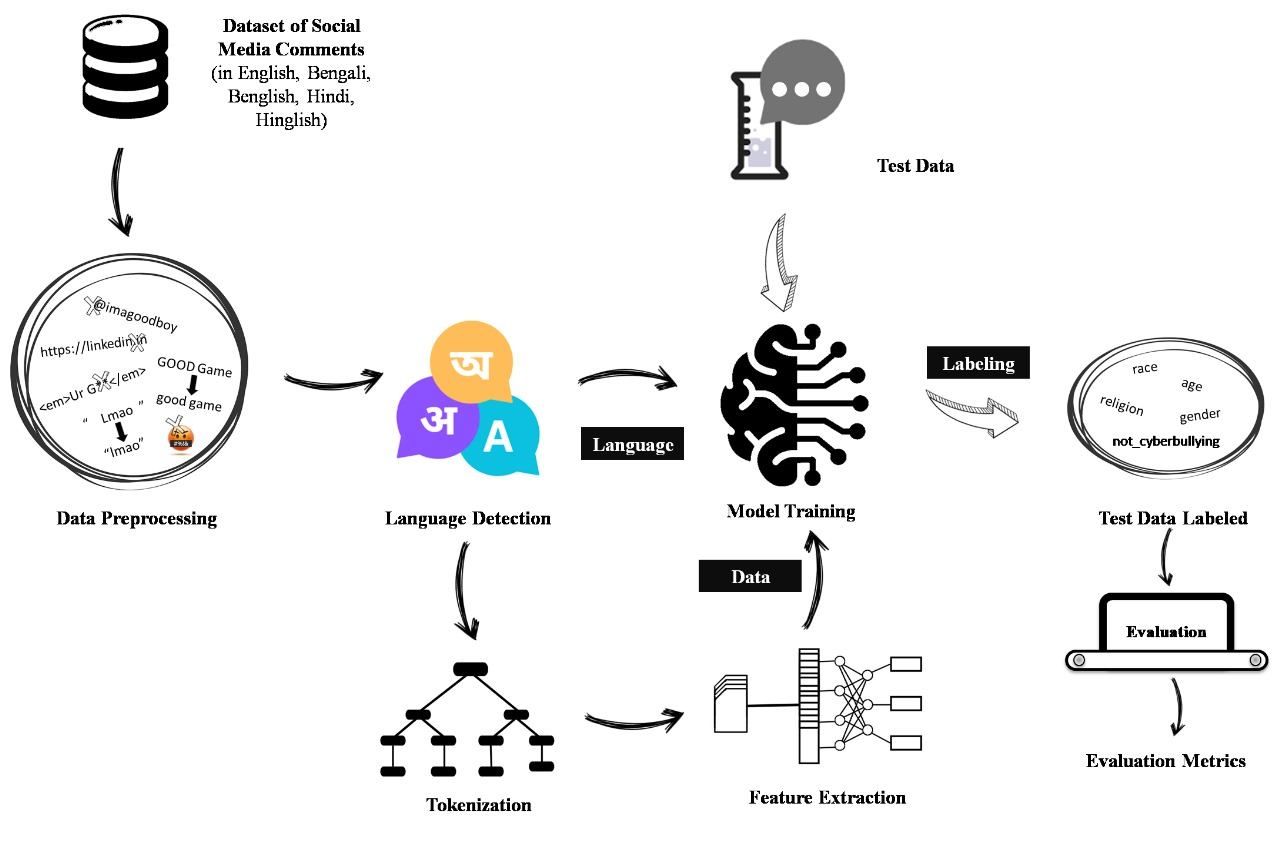
\includegraphics[width=0.95\textwidth]{Graphs/flowchart2.jpg}
    \caption{Flowchart of the model}
    \label{fig:flowchart}
\end{figure}

% \\The text cleaning steps included converting all text to lowercase, removing URLs, HTML tags, and usernames, as well as eliminating emojis and extra whitespaces.
% The dataset was split into 80\% training and 20\% testing sets using stratified sampling.

% A complete preprocessing step refined textual data before classification algorithms started to run. The sequential cleaning steps were implemented to the \texttt{text} column as follows:

% \begin{itemize}
%     \item \textbf{Lowercasing:} The conversion to lowercase characters solved replication issues generated by differing text format styles.
%     \item \textbf{URL and HTML tag removal:} Regular expressions extracted URLs and HTML tags to prevent analysis bias.
%     \item \textbf{Username and mention removal:} Removed user mentions or usernames like \texttt{@user} to prevent bias.
%     \item \textbf{Whitespace normalization:} Replaced repeated spaces with a single space for text uniformity.
%     \item \textbf{Emoji removal:} Eliminated Unicode symbols and emojis to ensure uniform character set.
% \end{itemize}

\subsection{Methodology and Result}


% The analysis of cyberbullying detection models utilized a complete processing framework that involved data preparation followed by algorithm development then assessment of ten different methods including classic machine learning solutions and deep neural networks and transformer modules.

The hybrid model pipeline contains three essential operational modules. Before analysis all input tweets undergo language detection to determine their language from English, Hindi, Bengali and Hinglish or Benglish. The Sentiment and Emotion Fusion Layer examines each sentiment-tagged comment by applying pretrained detection engines for sentiment analysis and emotions. Programming codes receive the output as feature vectors. A cyberbullying Classifier utilizes features from extracted data as input for ensembling three algorithms including Logistic Regression, Random Forest, and XGBoost models. The method included cross-validation to validate generalization capabilities.

%\subsubsection{Data Preparation and Preprocessing}

%The dataset consisted of user comments labeled either as \texttt{not\_cyberbullying} or with one of several cyberbullying categories: \texttt{age}, \texttt{race}, \texttt{gender}, \texttt{religion}.  The six binary columns were derived from the original label column in order to represent each possible category. The single-point value of one was assigned to the relevant category field and all other fields received a value of zero for each row.

%Text cleaning steps included:
%\begin{itemize}
 %   \item Converting all text to lowercase
  %  \item Removing URLs, HTML tags, and usernames
   % \item Removing emojis and extra whitespaces
%\end{itemize}

%The dataset was split into 80\% training and 20\% testing sets using stratified sampling.

\subsubsection{Algorithm}

% The following algorithm outlines the steps involved in the cyberbullying detection pipeline:

\begin{algorithmic}
\State \textbf{Input:} Raw Social Media Comments Datasets which include comments from Facebook, Instagram and X(Formerly Twitter) in English, Bengali, Benglish, Hindi and Hinglish.
\State \textbf{Output:} Binary or Multi-class classification.

\State \textbf{Step 1: Data Preprocessing}
\State The process starts by removing all mentions together with addresses, HTML components and Unicode exceptions.
\State Convert text to lowercase.
\State Normalize whitespace.
\State Detect language (fastText or langDetect).
\State The text requires tokenization through IndicBERT or mBERT as a multilingual tokenizer.

\State \textbf{Step 2: Feature Extraction}
\State Sentiment analysis requires VADER and BERT-sentiment model as analysis tools.
\State The system employs DistilBERT which received emotion detection training from emotion datasets to perform analysis.

\State \textbf{Step 3: Model Training}
\State The CNN requires text embeddings as an input to perform spatial feature extraction.
\State An Augmented BERT model should be trained to extract contextual features.
\State The Ensemble Classifier uses Random Forest together with XGBoost and Logistic Regression to combine its output results.

\State \textbf{Step 4: Prediction \& Classification}
\State An overall classification rating gets generated for each posted comment.
\State The model identifies cyberbullying when it occurs through various categories and other specified as non\_cyberbullying.


\end{algorithmic}
\\
\textbf{ }
\\
\begin{algorithmic}
\State \textbf{BERT Equation}
\\
\State BERT fine-tuning is done by minimizing the binary cross-entropy loss for each label:

\textbf{BERT Pre-training Loss Function}

The total BERT loss \( \mathcal{L}_{\text{BERT}} \) is the sum of the Masked Language Modeling (MLM) loss and the Next Sentence Prediction (NSP) loss:
\\
\[
\mathcal{L}_{\text{BERT}} = \mathcal{L}_{\text{MLM}} + \mathcal{L}_{\text{NSP}}
\]
\\
\textbf{1. Masked Language Modeling (MLM) Loss}

Let \( \mathcal{M} \subset \{1, 2, \dots, n\} \) be the set of masked token positions in an input sequence \( x = \{x_1, x_2, \dots, x_n\} \). The MLM loss is:
\\
\[
\mathcal{L}_{\text{MLM}} = - \sum_{i \in \mathcal{M}} \log P(x_i \mid x_{\setminus i})
\]

\textbf{2. Next Sentence Prediction (NSP) Loss}
\\
Let \( y \in \{0, 1\} \) be the NSP label (1 = next sentence, 0 = not next), and \( p \) be the predicted probability from the NSP classifier (typically from the [CLS] token output). Then:
\\
\[
\mathcal{L}_{\text{NSP}} = - \left[ y \log(p) + (1 - y) \log(1 - p) \right]
\]
\\
\textbf{Combined Loss}
\\
\[
\mathcal{L}_{\text{BERT}} = - \sum_{i \in \mathcal{M}} \log P(x_i \mid x_{\setminus i}) - \left[ y \log(p) + (1 - y) \log(1 - p) \right]
\]

\end{algorithmic}
% \textbf{1. Data Pre-processing:} Includes removal of user mentions, URLs, HTML tags, and Unicode anomalies, convertion of all text to lowercase, whitespace normalization and Language Detection using \texttt{fastText} or \texttt{langdetect} slong with Tokenizing text using \texttt{IndicBERT} or \texttt{mBERT}.  \\
% \text{ } \\
% \textbf{2. Feature Extraction:}  Performed sentiment analysis using \texttt{VADER} and \texttt{BERT-Sentiment} and Emotion Detection using \texttt{DistilBERT}. Encoded demographic markers (age, gender, religion, race).  \\

% \begin{algorithmic}
% \[
% \mathcal{L}_{\text{BERT}} = - \sum_{i \in \mathcal{M}} \log P(x_i \mid x_{\setminus i}) - \left[ y \log(p) + (1 - y) \log(1 - p) \right]
% \]
% \end{algorithmic}

% \text{ } \\
% \textbf{3. Model Training:} Used \texttt{CNN} for spatial feature extraction on text embeddings, Augmented \texttt{BERT} for contextual understanding, ensembled Random Forest, XGBoost, and Logistic Regression for final classification. \\
% \text{ } \\
% \textbf{4. Prediction \& Output:} Generated classification for each comment. Labeled as cyberbullying (with category) or non-cyberbullying. \\

\textbf{1. Data Pre-processing:} Used regex for cleaning, lowercase + whitespace normalization, language detection via \texttt{fastText}/\texttt{langdetect}, and tokenization with \texttt{IndicBERT}/\texttt{mBERT}.

\text{ } \\
\textbf{2. Feature Extraction:} Applied sentiment analysis using \texttt{VADER} and \texttt{BERT-Sentiment}, and emotion detection using \texttt{DistilBERT}. Among all, \texttt{BERT} yielded the most effective feature representations.

\text{ } \\
\textbf{3. BERT-based Decision Mechanism:} \texttt{BERT} captures contextual dependencies to identify semantic clues from comments and classifies them based on learned patterns of cyberbullying behavior. The loss function combines masked language modeling and binary classification as:

\[
\mathcal{L}_{\text{BERT}} = - \sum_{i \in \mathcal{M}} \log P(x_i \mid x_{\setminus i}) - \left[ y \log(p) + (1 - y) \log(1 - p) \right]
\]

where \( \mathcal{M} \) denotes the masked token positions, \( x_i \) the original tokens, and \( p \) the predicted probability for binary cyberbullying classification.

\text{ } \\
\textbf{4. Exit:} Output generated as cyberbullying (with category) or non-cyberbullying for each comment.


\text{ } \\
\textbf{Notations}
\begin{itemize}
    \item $\mathcal{L}_{\text{BERT}}$: Total loss function used in BERT.
    \item $\sum_{i \in \mathcal{M}}$: Summation over the set $\mathcal{M}$, the indices of masked tokens.
    \item $x_i$: The true token at position $i$.
    \item $x_{\backslash i}$: The input sequence excluding token at position $i$.
    \item $P(x_i \mid x_{\backslash i})$: Probability of token $x_i$ given the context $x_{\backslash i}$.
    \item $y$: Ground truth label for Next Sentence Prediction (NSP), $y \in \{0, 1\}$.
    \item $p$: Predicted probability that the second sentence follows the first one.
    \item $y \log(p) + (1 - y)\log(1 - p)$: Binary cross-entropy loss for NSP.
\end{itemize}


\subsubsection{Model Implementation}

The evaluation included distinct algorithms where the TF-IDF feature vectors trained Logistic Regression alongside Naive Bayes and Support Vector Machine (SVM) and Decision Tree and Random Forest and XGBoost. The research implemented Deep learning models adopting CNN alongside LSTM and GRU structures. The Hugging Face Transformers library was used to fine-tune BERT (base, uncased) as a transformer model. All models were optimized for multi-label classification using binary cross-entropy loss and evaluated using Subset Accuracy.

\clearpage

\subsubsection{Results}

Table \ref{tab:detailed_metrics} presents detailed performance metrics—precision, recall, and F1-score—across five protected attributes: age, race, gender, religion, and not\_cyberbullying, for each algorithm.

\begin{table}[h!]
\centering
\resizebox{\textwidth}{!}{%
\begin{tabular}{|l||c|c|c||c|c|c||c|c|c||c|c|c||c|c|c|}
\hline
\textbf{Model} & \multicolumn{3}{c||}{\textbf{age}} & \multicolumn{3}{c||}{\textbf{race}} & \multicolumn{3}{c||}{\textbf{gender}} & \multicolumn{3}{c||}{\textbf{religion}} & \multicolumn{3}{c|}{\textbf{not\_cyberbullying}} \\
& \textbf{prec.} & \textbf{recall} & \textbf{f1-score} & \textbf{prec.} & \textbf{recall} & \textbf{f1-score} & \textbf{prec.} & \textbf{recall} & \textbf{f1-score} & \textbf{prec.} & \textbf{recall} & \textbf{f1-score} & \textbf{prec.} & \textbf{recall} & \textbf{f1-score} \\
\hline
Logistic Regression & 0.9594 & 0.9462 & 0.9528 & 0.982 & 0.9474 & 0.9644 & 0.9566 & 0.8014 & 0.8722 & 0.9628 & 0.916 & 0.9389 & 0.8353 & 0.7944 & 0.8143 \\
Naive Bayes         & 0.9484 & 0.8974 & 0.9222 & 0.9753 & 0.8304 & 0.8971 & 0.9634 & 0.7171 & 0.8222 & 0.9312 & 0.8883 & 0.9092 & 0.8249 & 0.2999 & 0.4399 \\
SVM                 & 0.9733 & 0.9586 & 0.965  & 0.9813 & 0.9722 & 0.9767 & 0.9632 & 0.8196 & 0.874  & 0.9652 & 0.9268 & 0.9456 & 0.8232 & 0.8207 & 0.8219 \\
Decision Tree       & 0.9754 & 0.9675 & 0.9714 & 0.9752 & 0.9722 & 0.9737 & 0.8606 & 0.8456 & 0.853  & 0.9302 & 0.9261 & 0.9282 & 0.7798 & 0.7931 & 0.7864 \\
Random Forest       & 0.9873 & 0.9712 & 0.9792 & 0.9918 & 0.974  & 0.9828 & 0.9251 & 0.9332 & 0.8767 & 0.9457 & 0.9451 & 0.9454 & 0.828  & 0.8219 & 0.8249 \\
XGBoost             & 0.9929 & 0.9675 & 0.9808 & 0.9888 & 0.979  & 0.9838 & 0.9509 & 0.8293 & 0.886  & 0.9486 & 0.9765 & 0.9624 & 0.7966 & 0.9051 & 0.8476 \\
CNN                 & 0.9817 & 0.9725 & 0.9771 & 0.9887 & 0.9759 & 0.9822 & 0.9109 & 0.8553 & 0.8822 & 0.9471 & 0.9375 & 0.9422 & 0.8623 & 0.8066 & 0.8184 \\
LSTM                & 0.9589 & 0.9691 & 0.9639 & 0.9829 & 0.9816 & 0.9822 & 0.9193 & 0.8433 & 0.8796 & 0.9554 & 0.9607 & 0.958  & 0.8048 & 0.8761 & 0.8392 \\
GRU                 & 0.967  & 0.9767 & 0.9719 & 0.9829 & 0.9816 & 0.9822 & 0.9277 & 0.8446 & 0.8842 & 0.9615 & 0.9352 & 0.9482 & 0.812  & 0.8612 & 0.8359 \\
BERT                & 0.9872 & 0.9789 & \textbf{0.9863} & 0.9964 & 0.9812 & \textbf{0.9844} & 0.9232 & 0.9125 & \textbf{0.9136} & 0.951  & 0.9601 & \textbf{0.9623} & 0.8612 & 0.8876 & \textbf{0.8678} \\
\hline
\end{tabular}%
}
\caption{Detailed classification metrics of different models for protected attributes}
\label{tab:detailed_metrics}
\end{table}



Table \ref{tab:subset_accuracy} presents the Subset Accuracy achieved by each algorithm on the test dataset.

\begin{table}[h!]
\centering
\begin{tabular}{|l|c|}
\hline
\textbf{Algorithm} & \textbf{Subset Accuracy} \\
\hline
Logistic Regression & 0.7926 \\
Naive Bayes         & 0.7228 \\
SVM                 & 0.8928 \\
Decision Tree       & 0.8722 \\
Random Forest       & 0.9047 \\
XGBoost             & 0.9171 \\
CNN                 & 0.8930 \\
LSTM                & 0.9066 \\
GRU                 & 0.9068 \\
BERT                & \textbf{0.9416} \\
\hline
\end{tabular}
\caption{Subset Accuracy of various models for cyberbullying detection}
\label{tab:subset_accuracy}
\end{table}


\subsubsection{Visual Results for Each Algorithm}
Figures below provide comparative visual insights into the performance of each algorithm used in the study.

\begin{figure}[H]
    \begin{minipage}{0.48\textwidth}
        \centering
        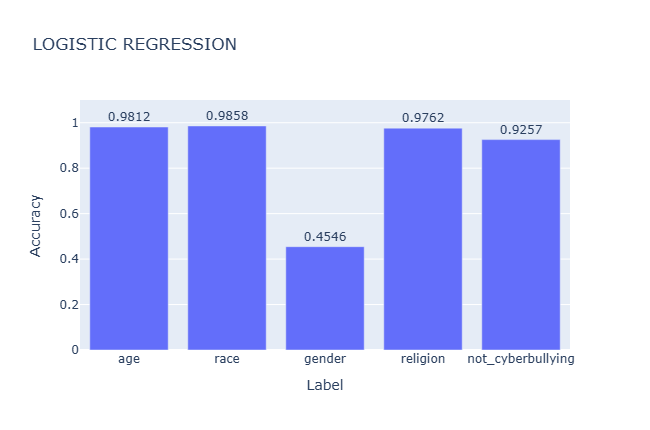
\includegraphics[width=\textwidth]{Graphs/LOGISTIC REGRESSION.png}
        \caption{Performance of Logistic Regression}
        \label{fig:logistic_regression}
    \end{minipage}
    \hfill
    \begin{minipage}{0.48\textwidth}
        \centering
        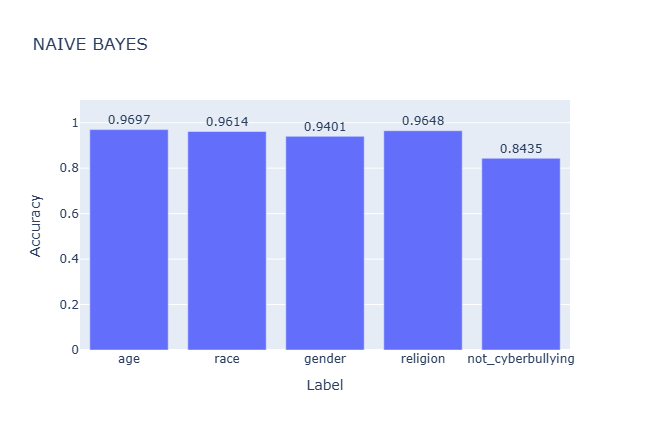
\includegraphics[width=\textwidth]{Graphs/NAIVE BAYES.png}
        \caption{Performance of Naive Bayes}
        \label{fig:naive_bayes}
    \end{minipage}
\end{figure}

\begin{figure}[H]
    \begin{minipage}{0.48\textwidth}
        \centering
        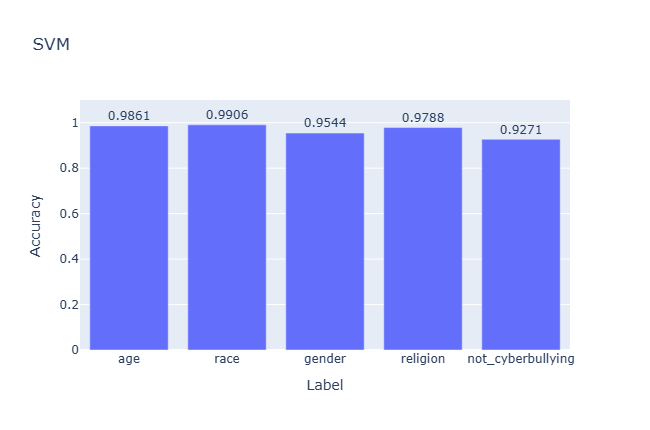
\includegraphics[width=\textwidth]{Graphs/SVM.png}
        \caption{Performance of SVM}
        \label{fig:svm}
    \end{minipage}
    \hfill
    \begin{minipage}{0.48\textwidth}
        \centering
        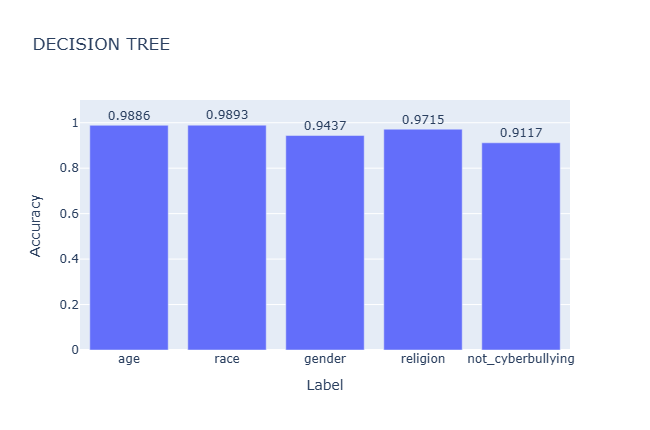
\includegraphics[width=\textwidth]{Graphs/DECISION TREE.png}
        \caption{Performance of Decision Tree}
        \label{fig:decision_tree}
    \end{minipage}
\end{figure}

\begin{figure}[H]
    \begin{minipage}{0.48\textwidth}
        \centering
        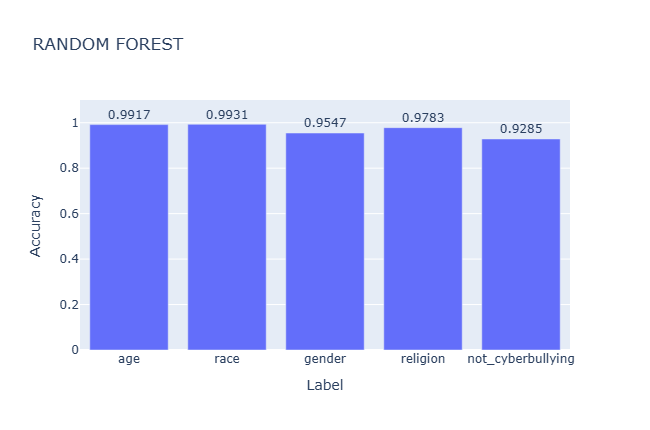
\includegraphics[width=\textwidth]{Graphs/RANDOM FOREST.png}
        \caption{Performance of Random Forest}
        \label{fig:random_forest}
    \end{minipage}
    \hfill
    \begin{minipage}{0.48\textwidth}
        \centering
        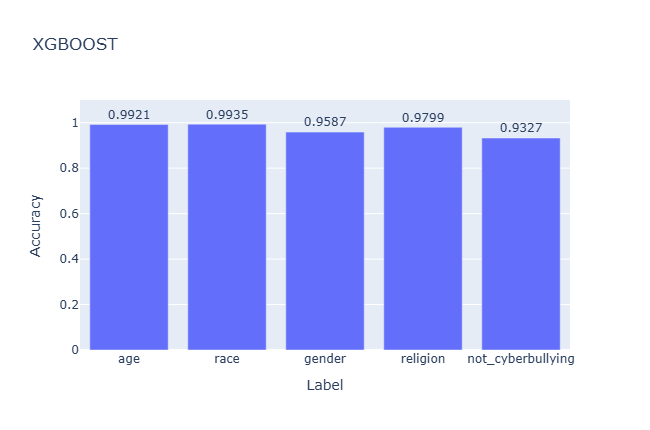
\includegraphics[width=\textwidth]{Graphs/XGBOOST.png}
        \caption{Performance of XGBoost}
        \label{fig:xgboost}
    \end{minipage}
\end{figure}

\begin{figure}[H]
    \begin{minipage}{0.48\textwidth}
        \centering
        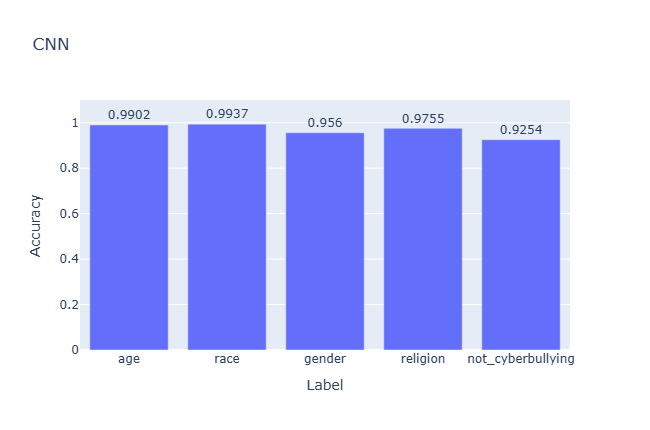
\includegraphics[width=\textwidth]{Graphs/CNN.png}
        \caption{Performance of CNN}
        \label{fig:cnn}
    \end{minipage}
    \hfill
    \begin{minipage}{0.48\textwidth}
        \centering
        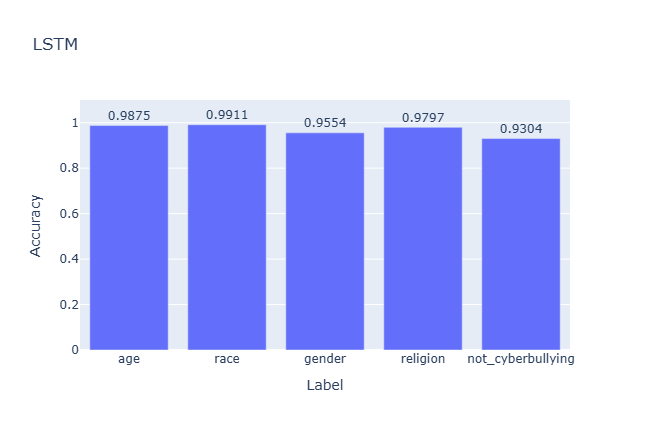
\includegraphics[width=\textwidth]{Graphs/LSTM.png}
        \caption{Performance of LSTM}
        \label{fig:lstm}
    \end{minipage}
\end{figure}

\begin{figure}[H]
    \begin{minipage}{0.48\textwidth}
        \centering
        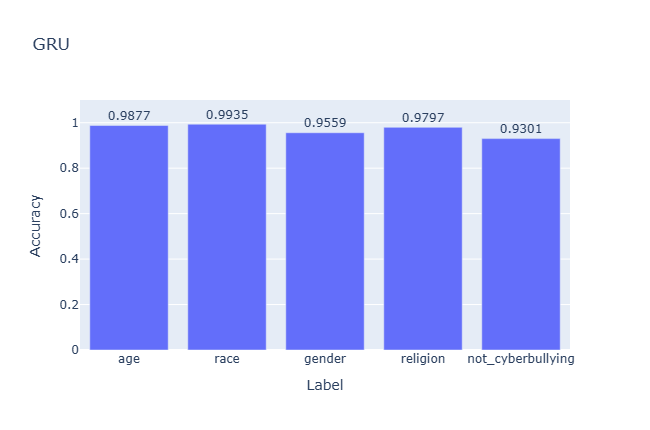
\includegraphics[width=\textwidth]{Graphs/GRU.png}
        \caption{Performance of GRU}
        \label{fig:gru}
    \end{minipage}
    \hfill
    \begin{minipage}{0.48\textwidth}
        \centering
        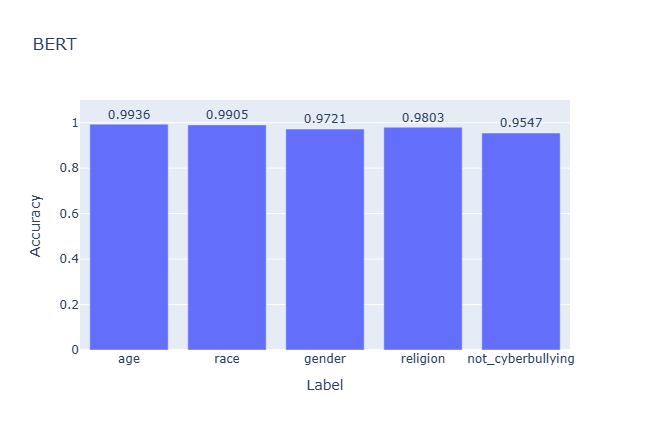
\includegraphics[width=\textwidth]{Graphs/BERT.png}
        \caption{Performance of BERT}
        \label{fig:bert}
    \end{minipage}
\end{figure}

\begin{figure}[H]
    \centering
    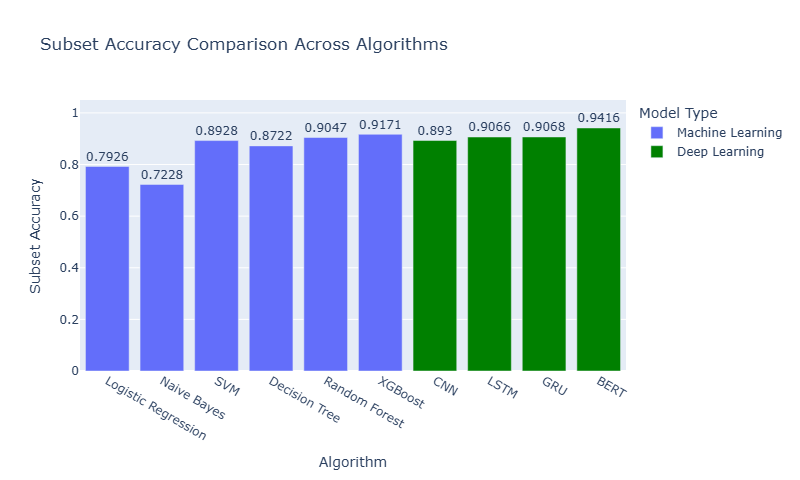
\includegraphics[width=0.95\textwidth]{Graphs/Subset Accuracy Comparison Across Algorithms.png}
    \caption{Subset Accuracy Comparison Across All Models}
    \label{fig:subset_accuracy_final}
\end{figure}


\subsubsection{Analysis}

The tested models revealed that \textbf{BERT} produced the highest performance by reaching a Subset Accuracy value of \textbf{0.9416} due to its efficient contextual analysis in multi-label tasks. The three most successful systems in this assessment were \textbf{XGBoost} with 0.9171 accuracy and \textbf{GRU} and \textbf{LSTM} reaching 0.9068 to 0.9066 respectively.
The \textbf{CNN} model displayed strong ability to detect local text patterns by reaching a Subset Accuracy value of 0.8930. The traditional ensemble techniques \textbf{SVM}, \textbf{Decision Tree} and \textbf{Random Forest} obtained high performance metrics (0.8928, 0.8722 and 0.9047 respectively), yet simpler algorithms demonstrated reduced success such as \textbf{Logistic Regression} with 0.7926 and \textbf{Naive Bayes} at 0.7228.The results underscore the advantage of deep learning, particularly transformer-based architectures in handling complex multi-label classification problems in cyberbullying detection.

% \clearpage 

\subsection{Discussion}

The prediction results for Logistic Regression together with Naive Bayes and several other models exhibit medium accuracy levels in Table \ref{tab:model_observations}. Support Vector Machines (SVM) deployed as part of ensemble methods with Random Forest and XGBoost achieves notable accuracy gains for the system. The deep learning models LSTM and GRU process sequential data with greater competence than traditional models, leading to more precise accuracy results. BERT transformer-based model reaches the highest accuracy level because it excels at contextual word interpretation. Complex text patterns are easier to detect through the Transformer architecture when systems perform analysis on cyberbullying content.

\begin{table}[htbp]
\centering
\begin{tabular}{|>{\centering\arraybackslash}m{3.5cm}|>{\centering\arraybackslash}m{2cm}|>{\raggedright\arraybackslash}m{6cm}|}
\hline
\textbf{Model} & \textbf{Accuracy} & \textbf{Observations} \\
\hline
Logistic Regression & 0.7926 & Performs reasonably well on structured data; limited in capturing textual context. \\
\hline
Naive Bayes & 0.7228 & Fast and simple; assumes feature independence which limits contextual understanding. \\
\hline
Support Vector Machine (SVM) & 0.8928 & Effective in high-dimensional spaces; sensitive to kernel and parameter tuning. \\
\hline
Decision Tree & 0.8722 & Interpretable; tends to overfit if not pruned or regularized. \\
\hline
Random Forest & 0.9047 & Reduces overfitting via ensemble learning; handles imbalanced data better. \\
\hline
XGBoost & 0.9171 & High accuracy and efficient; requires careful hyperparameter tuning. \\
\hline
CNN & 0.8930 & Captures local patterns in text effectively; lacks sequential understanding. \\
\hline
LSTM & 0.9066 & Excels at sequential data modeling; slower to train than CNN. \\
\hline
GRU & 0.9068 & Similar to LSTM but faster and slightly more efficient; handles long-term dependencies. \\
\hline
BERT (Transformer) & \textbf{0.9416} & Pre-trained contextual embeddings significantly improve performance; highest accuracy across all models. \\
\hline
\end{tabular}
\caption{Model-wise Performance and Observations}
\label{tab:model_observations}
\end{table}



\noindent


\section{Conclusion}
Social media cyberbullying continues to expand so researchers have developed detection systems which apply ML and DL technology to analyze linguistic and multichannel inputs for abusive content. The combination of network processing techniques with neural network technology enables identification of verbal along with coded and visual harassment. Preventing detection of covert offensive language proves difficult due to the presence of slang terms and abbreviations together with emoticons and memes. The contextual abilities of BERT-like models excel but they face difficulties when processing casual dialogue. Word innovations tend to evolve more quickly than natural language processing capabilities do. The available models exclusively target Twitter and Facebook while lacking flexibility in their design. The development of powerful systems that maintain stable performance dynamics across distinct user engagements depends on applying transfer learning to multi-platform database inputs.



% A social media platform threat grows steadily due to the expansion of cyberbullying incidents. Research showed how ML and DL algorithms operate in cyberbullying detection systems by using linguistic and multichannel inputs to identify abusive content. Traditional network processing when integrated with neural networks enables the monitoring of harassment patterns which include verbal as well as coded and visual content.

% Main obstacles persist in detecting hidden offensive language from non-standard expressions which include slang and shortened text combined with emoticons and meme-based communications. Recent word innovations appear faster than regular NLP models can track them. The current version of BERT-like models shows advanced contextual analysis but performs poorly in processing informal speech patterns. For effective detection the present frameworks need specialized pre-processing methods or new architectural frameworks.

% Current detection models focus exclusively on specific platforms such as Twitter and Facebook while they struggle to adjust their capabilities across various platforms that each have their own distinct user actions. To achieve accurate detection capabilities while maintaining model performance researchers must create adaptable models using transfer learning methods on diverse multi-platform data collections.
% Limited evidence exists regarding how cyberbullying impacts individuals psychologically and neurobiologically through depression and anxiety, together with alterations in neural activity. Early intervention strength increases alongside the implementation of behavioral analysis with sentiment metrics and psychological data that provides personalized assistance for both victims and aggressors. The deployment of smart detection systems creates multiple ethical problems along with privacy violations. System performance requires strict privacy safeguards along with fairness audits and explainable AI (XAI) to prevent flagging biases related to gender, race or language in order to maintain responsible, effective system performance.

% The research field dedicated to studying psychological and neurobiological impacts of cyberbullying through anxiety development and depression increase and neural system modification shows inadequate investigation. The integration of behavioral analysis with sentiment metrics alongside psychological assessment data enhances system detection capabilities so that both victim and aggressor receive early warning and tailored assistance.

% Smart detection systems create ethical problems alongside privacy problems due to their deployment. Clear processes alongside strict protection of privacy standards remain vital since algorithmic biases cause improper content flags that stem from gender, racial or language-based classification errors. AI system performance improves with responsible practices that include both fairness audits and explainable AI (XAI).

% The creation of an ideal cyberbullying detection system needs support at multiple levels from professionals who demonstrate expertise in computation as well as psychology and linguistics and follow ethical standards. Danger detection using deep learning models performs real-time cyberbullying surveillance of diverse content but needs additional development. The future development of cyberbullying prevention systems needs psychological indicators and ethical assessments combined with technician-sociologist-policymaker-psychiatrist collaboration to achieve secure and ethical mechanisms that prevent cyberbullying.

% The following phase of model development should concentrate on building systems capable of analyzing formal along with informal abusive content by incorporating psychological indicators for enhanced detection precision. The objective of achieving ethical analysis and decreasing detection system biases requires technological specialists to partner with psychiatrists sociologists and policymakers.

% The battle to eliminate cyberbullying involves more than implementing technical solutions. In order to achieve secure digital environments the world needs continuous creativity alongside ethical practices and unified goals.

% A subsequent development stage must include psychological markers to improve the identification of abusive content in all forms. The elimination of biases and ethical analysis needs technicians to work together with psychiatrists sociologists and policymakers. Secure digital environments will be achieved through continuous creative measures and unified efforts and ethical practices against cyberbullying.



\bibliography{sn-bibliography}% common bib file
%% if required, the content of .bbl file can be included here once bbl is generated
%%\input sn-article.bbl


\end{document}
